\documentclass[tikz,border=8pt]{standalone}
\usepackage{amsmath,amssymb}
\usetikzlibrary{arrows.meta,calc,decorations.pathreplacing,patterns,shapes.geometric,positioning,shadings}

\begin{document}
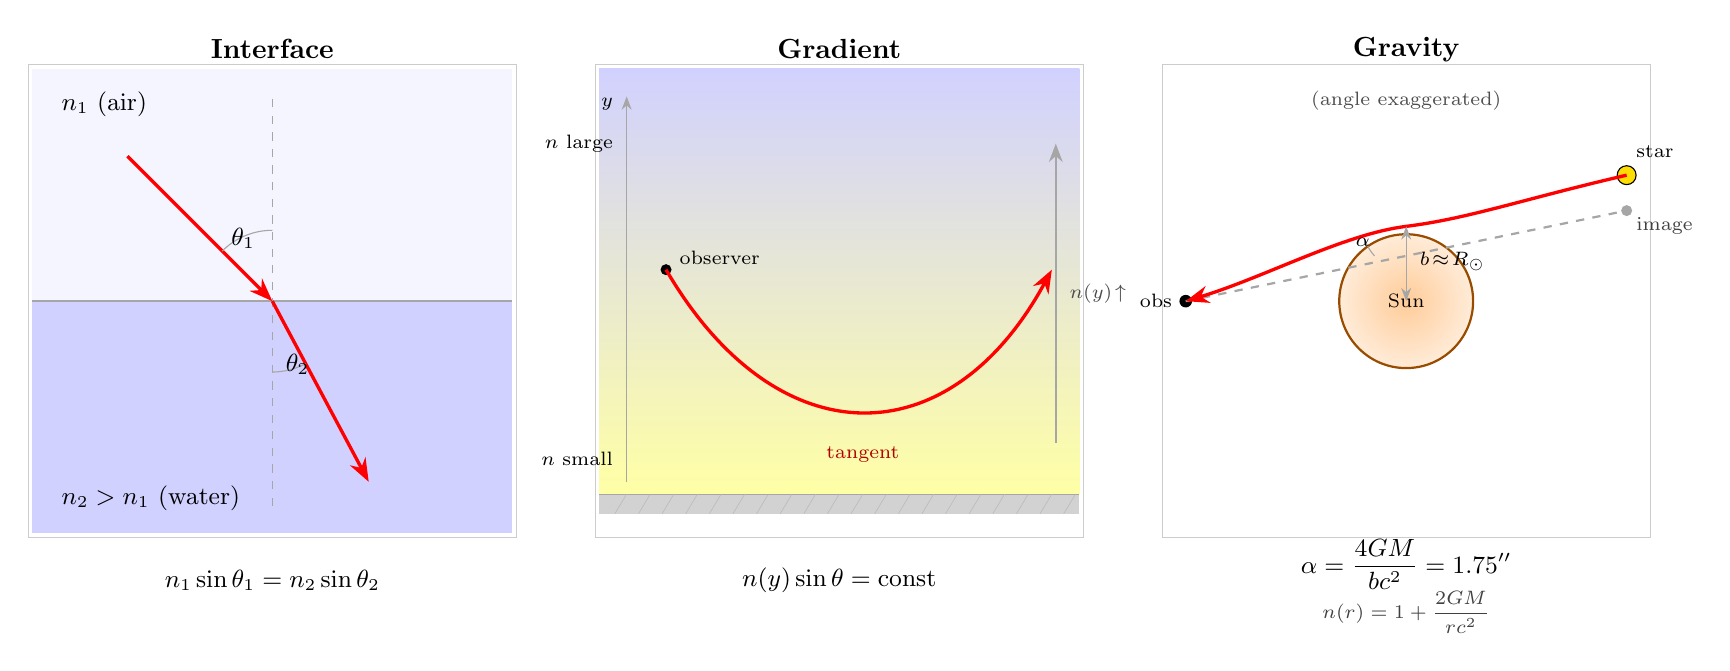
\begin{tikzpicture}[>=Stealth,font=\small]

% =====================================================
% Global layout: three panels
% Panel width ~6.2, heights ~6. Separated by vertical gaps
% =====================================================

% Panel titles row (top)
\node[font=\bfseries] at (3.1,6.2) {Interface};
\node[font=\bfseries] at (10.3,6.2) {Gradient};
\node[font=\bfseries] at (17.5,6.2) {Gravity};

% =====================================================
% PANEL 1 : Interface refraction (Snell's law)
% Frame: x in [0,6.2], y in [0,6]
% =====================================================
\begin{scope}[shift={(0,0)}]
  % panel border
  \draw[gray!40] (0,0) rectangle (6.2,6);

  % Upper medium n1 (lighter), lower medium n2 (darker, larger n)
  \fill[blue!4] (0.05,3) rectangle (6.15,5.95);
  \fill[blue!18] (0.05,0.05) rectangle (6.15,3);

  % Interface line
  \draw[thick,gray!70] (0.05,3) -- (6.15,3);

  % Normal (dashed)
  \draw[dashed,gray!70] (3.1,0.4) -- (3.1,5.6);

  % Incident ray (from upper-left, angle theta1 ~ 45 deg from normal)
  % Using sin45 = 0.707, choose theta1=45; by Snell with n1=1, n2=1.5 -> sin theta2 = 0.471 -> theta2 ~28.1
  % Incident direction unit: (sin45,-cos45)=(0.707,-0.707). Start so hits (3.1,3)
  % Length 2.6 -> start = (3.1 - 2.6*0.707, 3 + 2.6*0.707) = (1.26, 4.84)
  \draw[red,very thick,->] (1.26,4.84) -- (3.1,3);
  % Refracted: direction (sin28.1, -cos28.1) = (0.471,-0.882); length 2.6 -> end = (3.1+1.224, 3-2.294) = (4.324,0.706)
  \draw[red,very thick,->] (3.1,3) -- (4.324,0.706);

  % Angle arcs
  % theta1 arc between normal (upward from interface) and incident
  \draw[gray!70] (3.1,3) ++(90:0.9) arc (90:135:0.9);
  \node at (2.73,3.8) {$\theta_1$};
  % theta2 arc between normal (downward) and refracted
  \draw[gray!70] (3.1,3) ++(270:0.9) arc (270:298.1:0.9);
  \node at (3.42,2.2) {$\theta_2$};

  % Medium labels
  \node[anchor=west] at (0.3,5.5) {$n_1$ (air)};
  \node[anchor=west] at (0.3,0.5) {$n_2 > n_1$ (water)};

  % Formula
  \node[font=\small] at (3.1,-0.55) {$n_1\sin\theta_1 = n_2\sin\theta_2$};
\end{scope}

% =====================================================
% PANEL 2 : Continuous gradient (mirage)
% Frame: x in [7.2,13.4], y in [0,6]
% =====================================================
\begin{scope}[shift={(7.2,0)}]
  \draw[gray!40] (0,0) rectangle (6.2,6);

  % Vertical gradient: hot thin layer near ground (yellow, small n),
  % cooler above (light blue, larger n). Use explicit bands.
  \shade[top color=blue!18,bottom color=yellow!35]
     (0.05,0.55) rectangle (6.15,5.95);

  % Ground (concrete surface) at y=0.55
  \fill[gray!35] (0.05,0.3) rectangle (6.15,0.55);
  \draw[gray!70] (0.05,0.55) -- (6.15,0.55);
  % hatch pattern on ground
  \foreach \x in {0.25,0.55,...,6.05} {
    \draw[gray!55,very thin] (\x,0.3) -- ({\x+0.15},0.55);
  }

  % n(y) axis (vertical)
  \draw[->,gray!70] (0.4,0.7) -- (0.4,5.6);
  \node[anchor=east,font=\scriptsize] at (0.35,5.5) {$y$};
  \node[anchor=east,font=\scriptsize] at (0.35,5.0) {$n$ large};
  \node[anchor=east,font=\scriptsize] at (0.35,1.0) {$n$ small};

  % Observer (eye) on left at y=3.4
  \fill[black] (0.9,3.4) circle (0.07);
  \node[anchor=west,font=\scriptsize] at (0.95,3.55) {observer};

  % Curved ray: from eye going forward, curving down near ground,
  % reaching minimum y~0.65 around x=3.4, then curving up to right
  % Use a smooth parabola-like bezier
  \draw[red,very thick,->]
    (0.9,3.4) .. controls (2.3,1.0) and (4.5,1.0) .. (5.8,3.4);

  % Mark tangent-to-ground region (inverted ray) with small annotation
  \node[font=\scriptsize,red!70!black] at (3.4,1.05) {tangent};

  % Formula label below
  \node[font=\small] at (3.1,-0.55) {$n(y)\sin\theta = \mathrm{const}$};

  % Small arrow showing "n increases upward"
  \draw[->,gray!70,thick] (5.85,1.2) -- (5.85,5.0);
  \node[anchor=west,font=\scriptsize,gray!60!black] at (5.9,3.1) {$n(y)\!\uparrow$};

\end{scope}

% =====================================================
% PANEL 3 : Gravitational lensing
% Frame: x in [14.4,20.6], y in [0,6]
% =====================================================
\begin{scope}[shift={(14.4,0)}]
  \draw[gray!40] (0,0) rectangle (6.2,6);

  % Sun disk (pale orange), radius 0.85 centered at (3.1,3.0)
  \shade[inner color=orange!40,outer color=orange!15]
     (3.1,3.0) circle (0.85);
  \draw[orange!60!black,thick] (3.1,3.0) circle (0.85);
  \node[font=\scriptsize] at (3.1,3.0) {Sun};

  % Source star (far right)
  \fill[yellow!80!orange] (5.9,4.6) circle (0.12);
  \draw (5.9,4.6) circle (0.12);
  \node[anchor=west,font=\scriptsize] at (5.9,4.9) {star};

  % Observer on far left
  \fill[black] (0.3,3.0) circle (0.08);
  \node[anchor=east,font=\scriptsize] at (0.25,3.0) {obs};

  % Geometric straight path (dashed, apparent position)
  % Straight line from observer (0.3,3.0) to apparent position (5.9,4.0) -- goes above sun
  \draw[dashed,gray!70,thick] (0.3,3.0) -- (5.9,4.15);
  % Apparent image position marker
  \fill[gray!70] (5.9,4.15) circle (0.07);
  \node[anchor=west,font=\scriptsize,gray!50!black] at (5.9,3.95) {image};

  % Actual bent path (solid red), two segments meeting near sun edge
  % From real star (5.9,4.6) to a point near sun's upper edge (3.1,3.95 is top edge),
  % choose impact parameter b just above the sun: point P = (3.1,3.95)
  % First segment: star -> P (nearly straight, slightly curved)
  \draw[red,very thick]
    (5.9,4.6) .. controls (4.6,4.3) and (3.9,4.05) .. (3.1,3.95);
  % Deflection at P, going to observer at (0.3,3.0)
  \draw[red,very thick,->]
    (3.1,3.95) .. controls (2.3,3.85) and (1.3,3.3) .. (0.3,3.0);

  % Impact parameter b label
  \draw[<->,gray!70] (3.1,3.0) -- (3.1,3.95);
  \node[anchor=west,font=\scriptsize] at (3.15,3.5) {$b\!\approx\!R_\odot$};

  % Deflection angle alpha at point P (between straight extension and bent ray going to obs)
  % We show a small arc at P indicating angle alpha (exaggerated)
  \draw[gray!70] (3.1,3.95) ++(200:0.55) arc (200:223:0.55);
  \node[font=\scriptsize] at (2.55,3.75) {$\alpha$};

  % Formula / labels below
  \node[font=\small] at (3.1,-0.35)
    {$\alpha=\dfrac{4GM}{bc^{2}}=1.75''$};
  \node[font=\scriptsize,gray!50!black] at (3.1,-0.95)
    {$n(r)=1+\dfrac{2GM}{rc^{2}}$};

  % Exaggeration note
  \node[font=\scriptsize,gray!60!black] at (3.1,5.55)
    {(angle exaggerated)};

\end{scope}

\end{tikzpicture}
\end{document}
